\noindent
\section{On $d$-regular tree:}
\noindent We next consider the case of {\bf $d$-regular trees} for $d\geq 3$ (at least $2$ children apart from $1$ parent) with a
distinguished root index $0$ which acts as the initial sender. For
simplicity we give the root an out-degree of $(d-1)$ by attaching a virtual
``mother vertex'' to the root which is also a sender but has only one
offspring and is not counted in the estimation of sender nodes (this helps
us avoid handling the initial steps (i.e., when only the root is having the
message) differently from the later steps). Let $A_{l}\left( t\right) ,$ $%
0\leq l<k,$ be the number of nodes on the tree which have exactly $l$
packets at time $t$ and have a direct communication link to one of the
sender nodes at time $t$. Note that each of the so defined nodes has exactly
one connection to a sender node due to the tree structure and the initial
condition of having just one sender at the beginning. We get the following
 exact linear recursion for the expectation $a_{l}\left( t+1\right) :=\hat{%
E}\left( A_{l}\left( t+1\right) \right) $ at time $t+1:$%
\begin{eqnarray*}
\nonumber
a_{l}\left( t+1\right) &=&\frac{d-1}{d}a_{l}\left( t\right) +\frac{1}{d}% 
a_{l-1}\left( t\right) ,1\leq l\leq k-1 \\ \nonumber
a_{0}\left( t+1\right) &=&\frac{d-1}{d}a_{k-1}\left( t\right) +\frac{d-1}{d}%
a_{0}\left( t\right) \nonumber
\end{eqnarray*}%
Note that for the expected number of sender nodes $s_{t}$ at time $t$, we
have 
\begin{equation}
s_{t}=\sum\limits_{t^{\prime }<t}\frac{1}{d}a_{k-1}\left( t^{\prime }\right)
\end{equation}

The asymptotic rate of growth of the variables $\left\{ a_{i}\left( t\right)
\right\} $ as well as $s_{t}$ is entirely determined by the value of the
largest eigenvalue of the associated transition matrix. The maximal
eigenvalue of the associated characteristic polynomial is given by 
\begin{equation*}
\lambda _{\max }=\frac{d-1}{d}+\left( \frac{d-1}{d}\left( \frac{1}{d}\right)
^{k-1}\right) ^{\frac{1}{k}}=\frac{d-1+\left( d-1\right) ^{1/k}}{d}
\end{equation*}


% \begin{figure}[htpb]
% %\vspace{-.5cm}
%  \centering
%   \includegraphics[scale=0.31]{figs1/plot_reg_tree.eps}
%   %\vspace{-5mm}
%   \caption{\label{tree_ratio}(a) Rate of diffusion ($s_t$ - $s_{t-1}$) throughout the 
% whole duration of the diffusion process for a 5-regular tree. (b) Number of nodes at each stage of infection versus time for 
% complete graph of $1000$ nodes with $k=4$. Although the creation of infected nodes is slow initially, the number of partially infected nodes ($0<p<4$) increases rapidly. (inset) Magnified version of the same figure.}
% %\vspace{-.45cm}
%  \end{figure} 

{In figure \ref{chapter_5_fig1}(b) we draw the diffusion dynamics for a 5-regular tree and in the same figure we show that the
analytical estimate (obtained from equation 5.17) of diffusion rate closely resemble the empirical
observation. 
\if{0}
to the point where the first leaf node receives the full message. 
%At this point, the leaf nodes are the only non-sender nodes in the network which can only be infected by the nodes in the previous level.
Since the leaf nodes after getting infected have no other nodes to infect,  the dynamics
slows down as is evident in the  figure  - the impact of finiteness on 
diffusion conspicuously gets illustrated in figure \ref{tree_ratio}(a)) where we look into the difference of $s_t$ and $s_{t-1}$ throughout the 
whole duration of the diffusion process. We observe that the diffusion rate initially follows an increasing trend and then drops.
\fi
%We observe that the ratio quickly stabilizes to $\lambda_{max}$ (represented in the same figure) after initial few time steps hence supporting our theory.  
%This is followed by a drop in diffusion rate as by that time infection reaches the leaf nodes.}
%\todo{Why should $\lambda_{max}$ = 1, it should be near to 2, check carefully.}

%\noindent {\em d-regular graph}: 
%We further observe that our analytical estimate for $d$-regular trees could be extended for {\bf $d$-regular graph} as well. We
%observe that the analytical estimate closely follows the empirical
%observations as is evident from figure \ref{fig1}. 
\begin{figure}[htpb]
%\vspace{-.5cm}
 \centering
  \includegraphics[scale=0.4]{./texfiles/Chapter_3/epl/figs1/plot_reg_tree.eps}
  %\vspace{-5mm}
  \caption{\label{tree_ratio}(a) $\frac{t_{1}^{\hat p} - t_1}{t_1}$ versus $\bar p$ for a complete graph with $1000$ nodes and $k=4$.
  (b) Number of nodes at each stage of infection versus time for 
complete graph of $1000$ nodes with $k=4$. Although the creation of infected nodes is slow initially, the number of partially infected nodes ($0<l<4$) increases rapidly. 
(inset) Magnified version of the same figure.}
\vspace{.45cm}
 \end{figure} 


\medskip
